\section{Intel SGX Background}
\label{ch:background:SGX}

\begin{figure}[t]
  \centering
    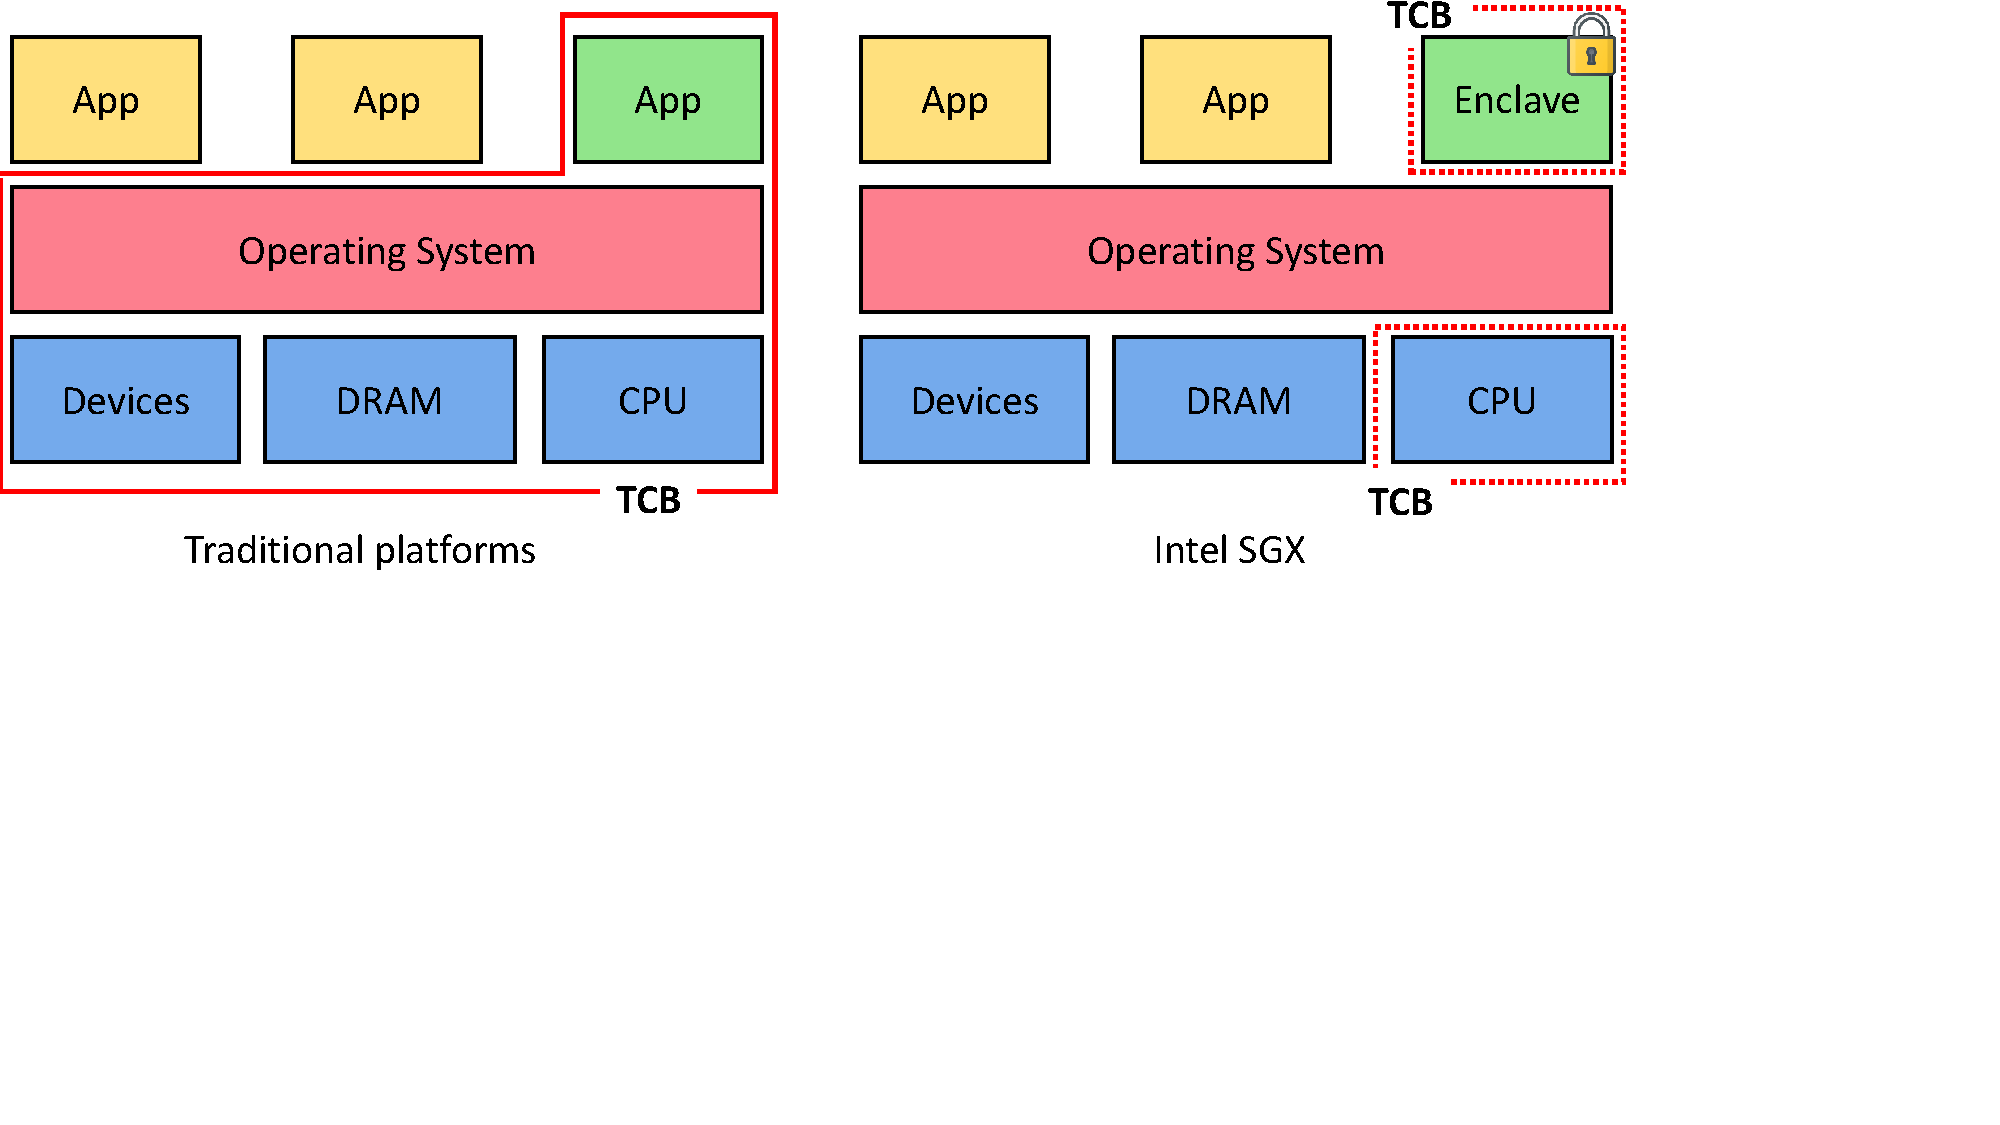
\includegraphics[trim={0 9cm 5cm 0},clip,width=\linewidth]{chapters/background/figures/SGX_trust.pdf}
    \caption[Intel SGX trust model compared to traditional platform]{\textbf{Intel SGX trust model compared to traditional platform.} The figure shows the comparison of software had hardware TCB between a traditional platform and an Intel SGX platform. In a traditional platform, the user of an application (e.g., the green app box) needs to trust the hardware (CPU, DRM, other devices, etc.) and the entire software stack (OS, VMM, hypervisor). Compared to the traditional platform, in an Intel SGX platform, the user needs to trust the specific isolated execution environment (enclave) and the Intel CPU.}
    \label{fig:sgx_trust_bg}
\end{figure}




Intel SGX is a TEE architecture that isolates application enclaves from all other software running on the system, including the privileged OS, hypervisor, BIOS etc.~\cite{costan2016intel}. Enclave's data is encrypted and integrity protected whenever it is moved outside the CPU chip. The untrusted OS is responsible for the enclave creation, and its initialization actions are recorded securely inside the CPU, creating a \emph{measurement} that captures the enclave's code. Enclaves can perform local attestation, which allows one enclave to ask the CPU to generate a signed report that includes its measurement. Another enclave on the same platform can verify the validity of the report without interacting with any other external services. Enclaves can \emph{seal} data to disk, which allows them to securely store confidential data such that only the same enclave running in the same CPU will be able to retrieve it later.



\subsection{Attestation}
\label{ch:background:SGX:attestation}

Attestation is an important security primitive for a TEE that ensures that the SGX platform runs a correct piece of software (enclave). Upon instantiation by the trusted hardware, the platform can compute the \emph{measurement} of the enclave that includes the cryptographic hash of the code, data, stack, heap, etc. The platform's private key then signs the measurement of the enclave. This signed measurement is known as the report. A verifier can then check the signature of the report to verify the following:

\begin{enumerate}
  \item The enclave is running on a legitimate platform.
  \item The enclave code is proper as it matches a known measurement of the software.
  \item Corresponding public key of the platform to create a secure channel with the enclave in order to provision secret to that enclave.
\end{enumerate}  

Intel SGX also implements an attestation scheme that follows the same principles. Every Intel processor comes with two device root keys that fused into the processor during the production phase~\cite{attestation_primitive} -  root provisioning key and root sealing key. These keys are the related key generations are shown in Figure~\ref{fig:keys_bg}. The attestation key is derived from these initial platform keys that are used to generate a report from the enclave measurement.


\begin{figure}[t]
  \centering
    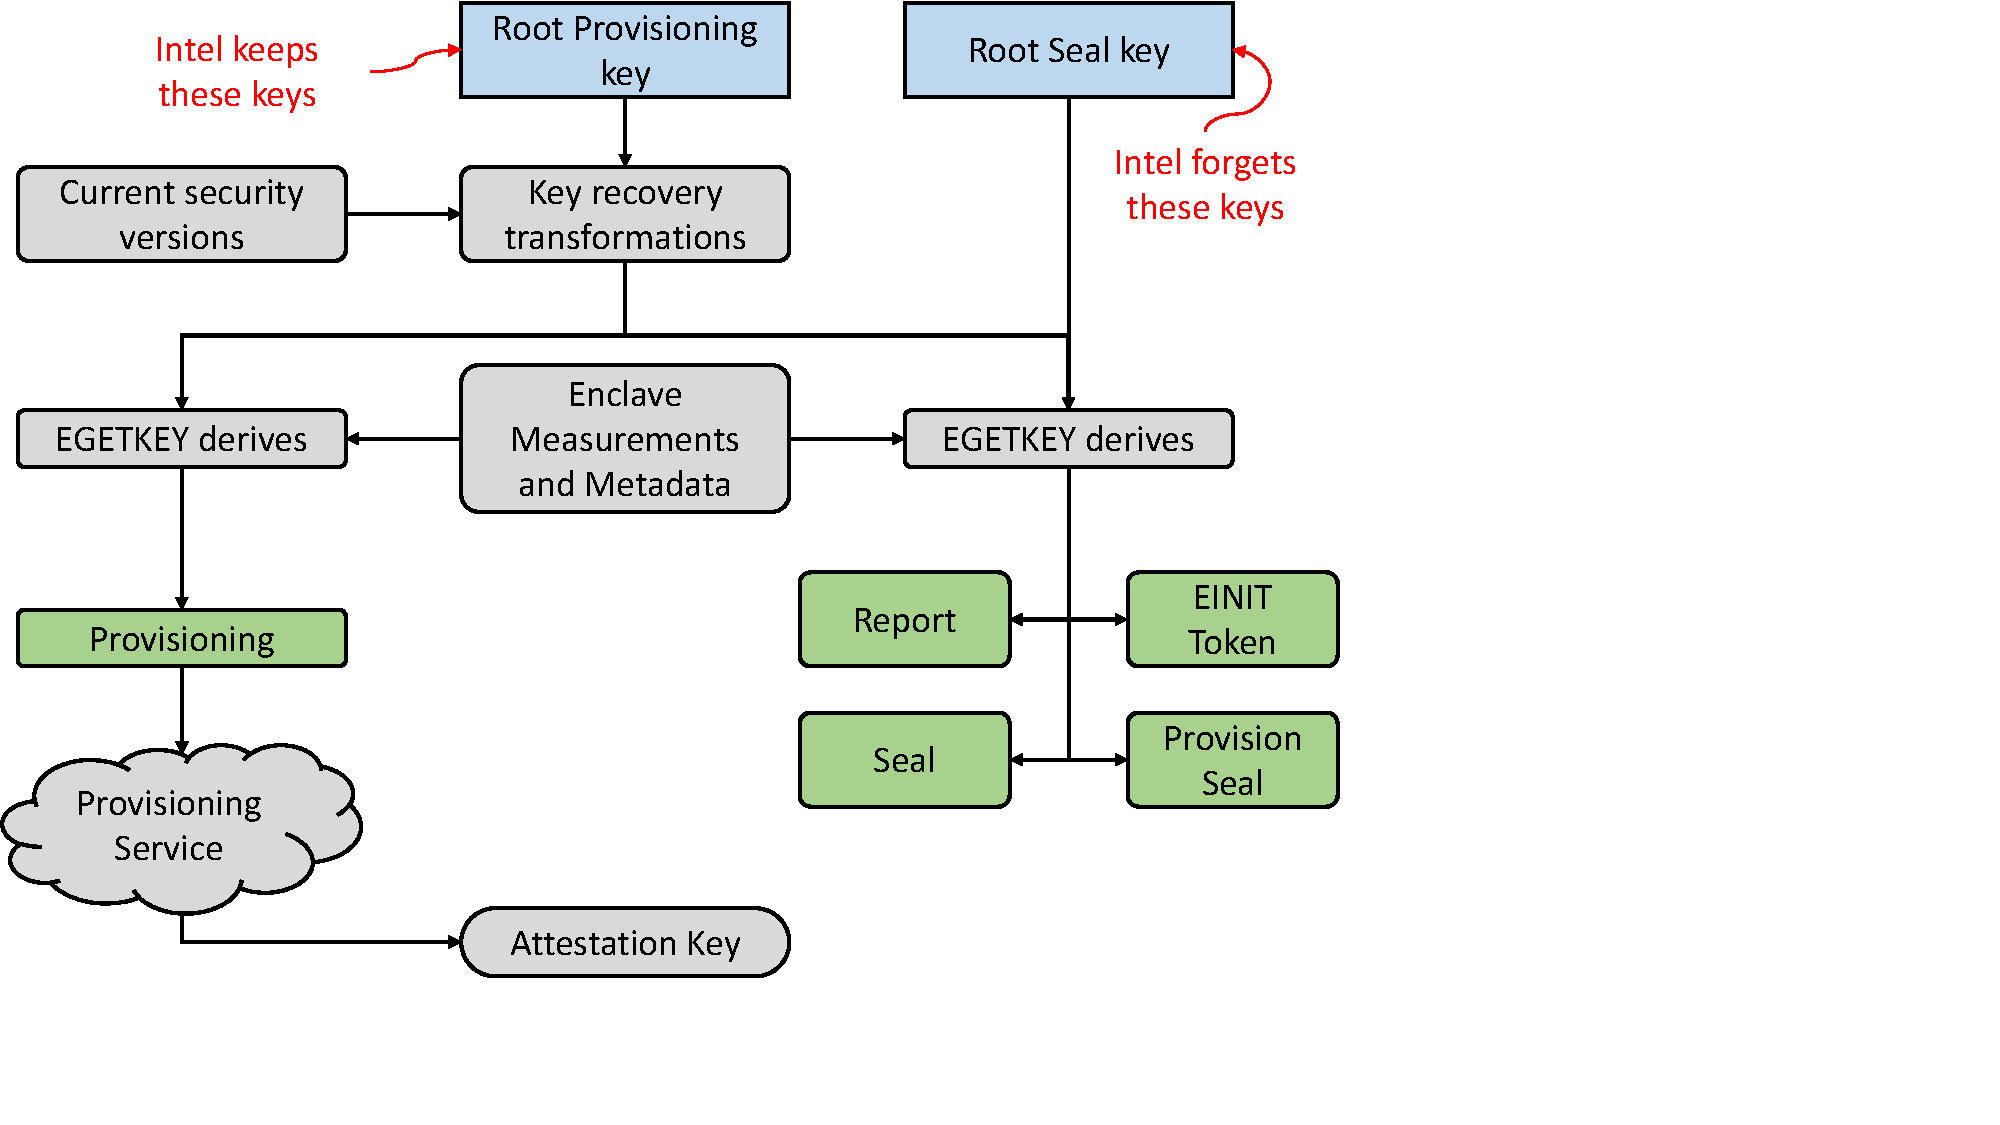
\includegraphics[trim={0 1cm 10cm 0},clip,width=0.9\linewidth]{chapters/background/figures/keys.pdf}
    \caption[Intel SGX keys and key derivations]{\textbf{Intel SGX keys and key derivations.} The figure shows the two platform keys: root provisioning key and root sealing key and their corresponding derived key for attestation and sealing. The figure is a reproduction of the official Intel documentation found in~\cite{attestation_primitive}.}
    \label{fig:keys_bg}
\end{figure}


\myparagraph{Measurement} When an enclave is built and initialized, Intel SGX will generate a cryptographic log of all the build activities (for more details, refer to Intel's white paper on attestation in sealing~\cite{attestation_primitive_all}), including:

\begin{itemize}
  \item The content of the enclave that includes code, data, stack, and heap
  \item Location of each page within the enclave
  \item Security flags being used
\end{itemize}
    
The "Enclave Identity", which is a 256-bit hash digest of the log, is stored as \texttt{MRENCLAVE} as the enclave's software TCB. In order to verify the software TCB, one should first securely obtain the enclave's software TCB, then securely obtain the expected enclave's software TCB and compare those two values.

\myparagraph{Report} \texttt{REPORT} contains the following information:

\begin{itemize}
  \item Measurement of the code and data in the enclave.
  \item A hash of the public key in the ISV certificate presented at enclave initialization time.
  \item User data.
  \item Other security-related state information.
  \item A signature block over the above data, which can be verified by the same platform that produced the report.
\end{itemize}

Intel SGX provides two forms of attestation: local attestation and remote attestation.


\begin{figure}[t]
  \centering
    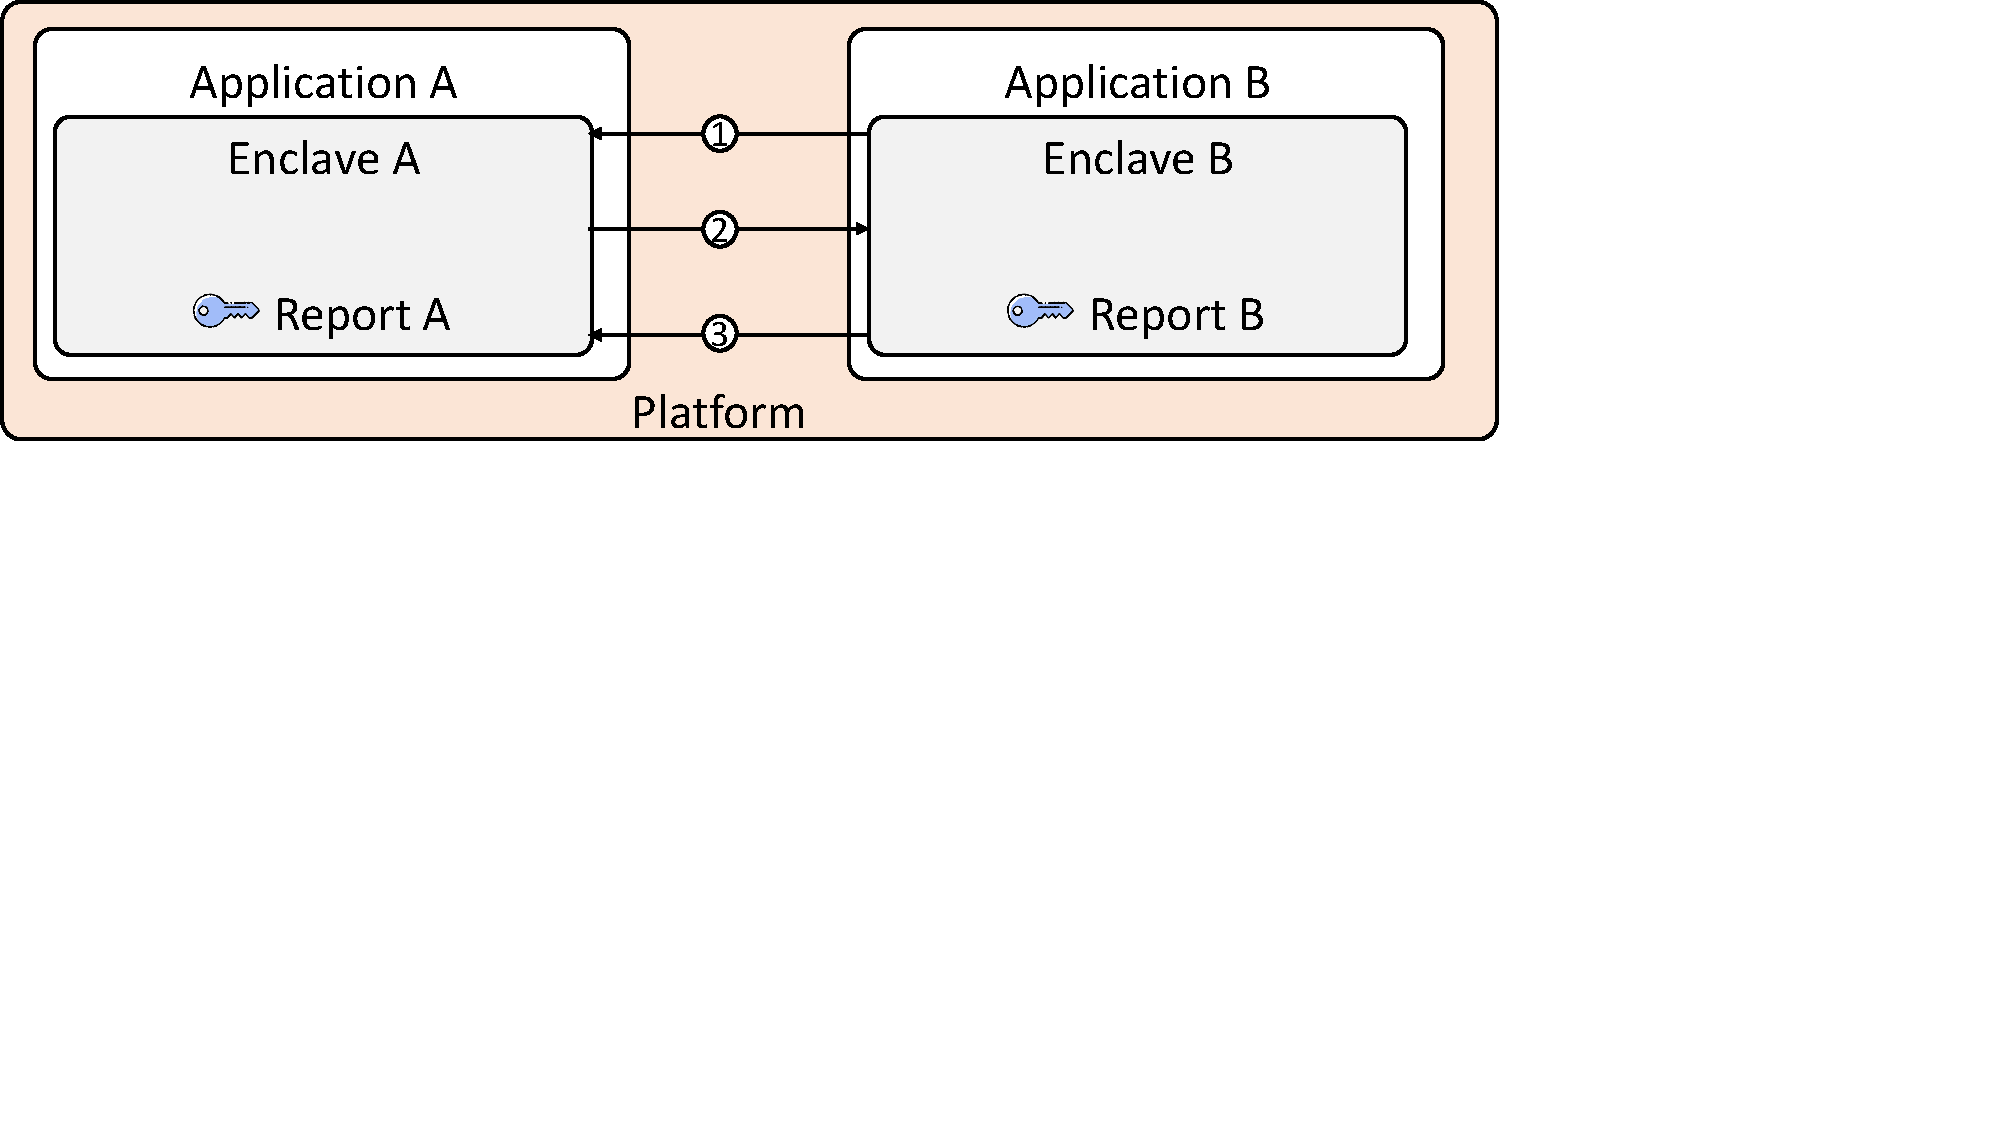
\includegraphics[trim={0 11cm 8cm 0},clip,width=0.9\linewidth]{chapters/background/figures/local_attestation.pdf}
    \caption[Intel SGX local attestation example]{\textbf{Intel SGXlocal attestation example.} Intel SGX local attestation example that involves two pairs of applications and enclaves (A and B). This figure is a reproduction of the figure in Intel's white paper~\cite{attestation_primitive_all}.}
    \label{fig:la_bg}
\end{figure}

\subsection{Local Attestation}
\label{ch:background:SGX:local}

Local attestation (also known as the Intra-Platform Attestation) enables two enclaves to verify that they are running the proper version of the enclave code on the same hardware platform. Figure~\ref{fig:la_bg} shows one such example of local attestation involving Application A that runs Enclave A and Application B that runs Enclave B. The step of the attestation process is as the following, and it follows the description provided in Intel's white paper~\cite{attestation_primitive_all}.

\begin{enumerate}
  \item [\one] Enclave A obtains Enclave B's \texttt{MRENCLAVE} value. We assume that Application A and Application B already have a communication channel over either shared memory or file system. Note that the actual communication channel does not have any effect on the local attestation process. Moreover, the communication channel between Application A and Application B does not need to be secure.
  \item [\two] Enclave A invokes the \texttt{EREPORT} instruction together with enclave B's \texttt{MRENCLAVE} to create a signed \texttt{REPORT} destined for enclave B. Enclave A transmits its \texttt{REPORT} to enclave B via the insecure communication channel mentioned in step \one.
  \item [\three] After receiving the \texttt{REPORT} from Enclave A, Enclave B executes the following steps:
  
   \begin{enumerate}
     \item  Enclave B calls \texttt{EGETKEY} to retrieve its Report Key, recomputes the \texttt{MAC} over the \texttt{REPORT} structure, and compares the result with the \texttt{MAC} accompanying the \texttt{REPORT}. A match in the \texttt{MAC} value confirms that A is indeed an enclave running on the same platform as Enclave B, and as such, Enclave A is running in an environment that abides by Intel SGX's security model.
     \item Once the firmware and hardware components of the TCB have been verified, and Enclave B can then examine Enclave A's \texttt{REPORT} to verify the software components of the TCB. \texttt{MRENCLAVE} reflects the contents of the software image running inside the enclave. \texttt{MRSIGNER} reflects the sealer's identity.
     \item Enclave B can then reciprocate by creating a \texttt{REPORT} for enclave A by using the \texttt{MRENCLAVE} value from the \texttt{REPORT} it just received.
     \item Enclave B transmits its \texttt{REPORT} to Enclave A. Enclave A can then similarly verify the report to enclave B, confirming that Enclave B exists on the same platform as Enclave A.
   \end{enumerate}
   
\end{enumerate}





\begin{figure}[t]
  \centering
    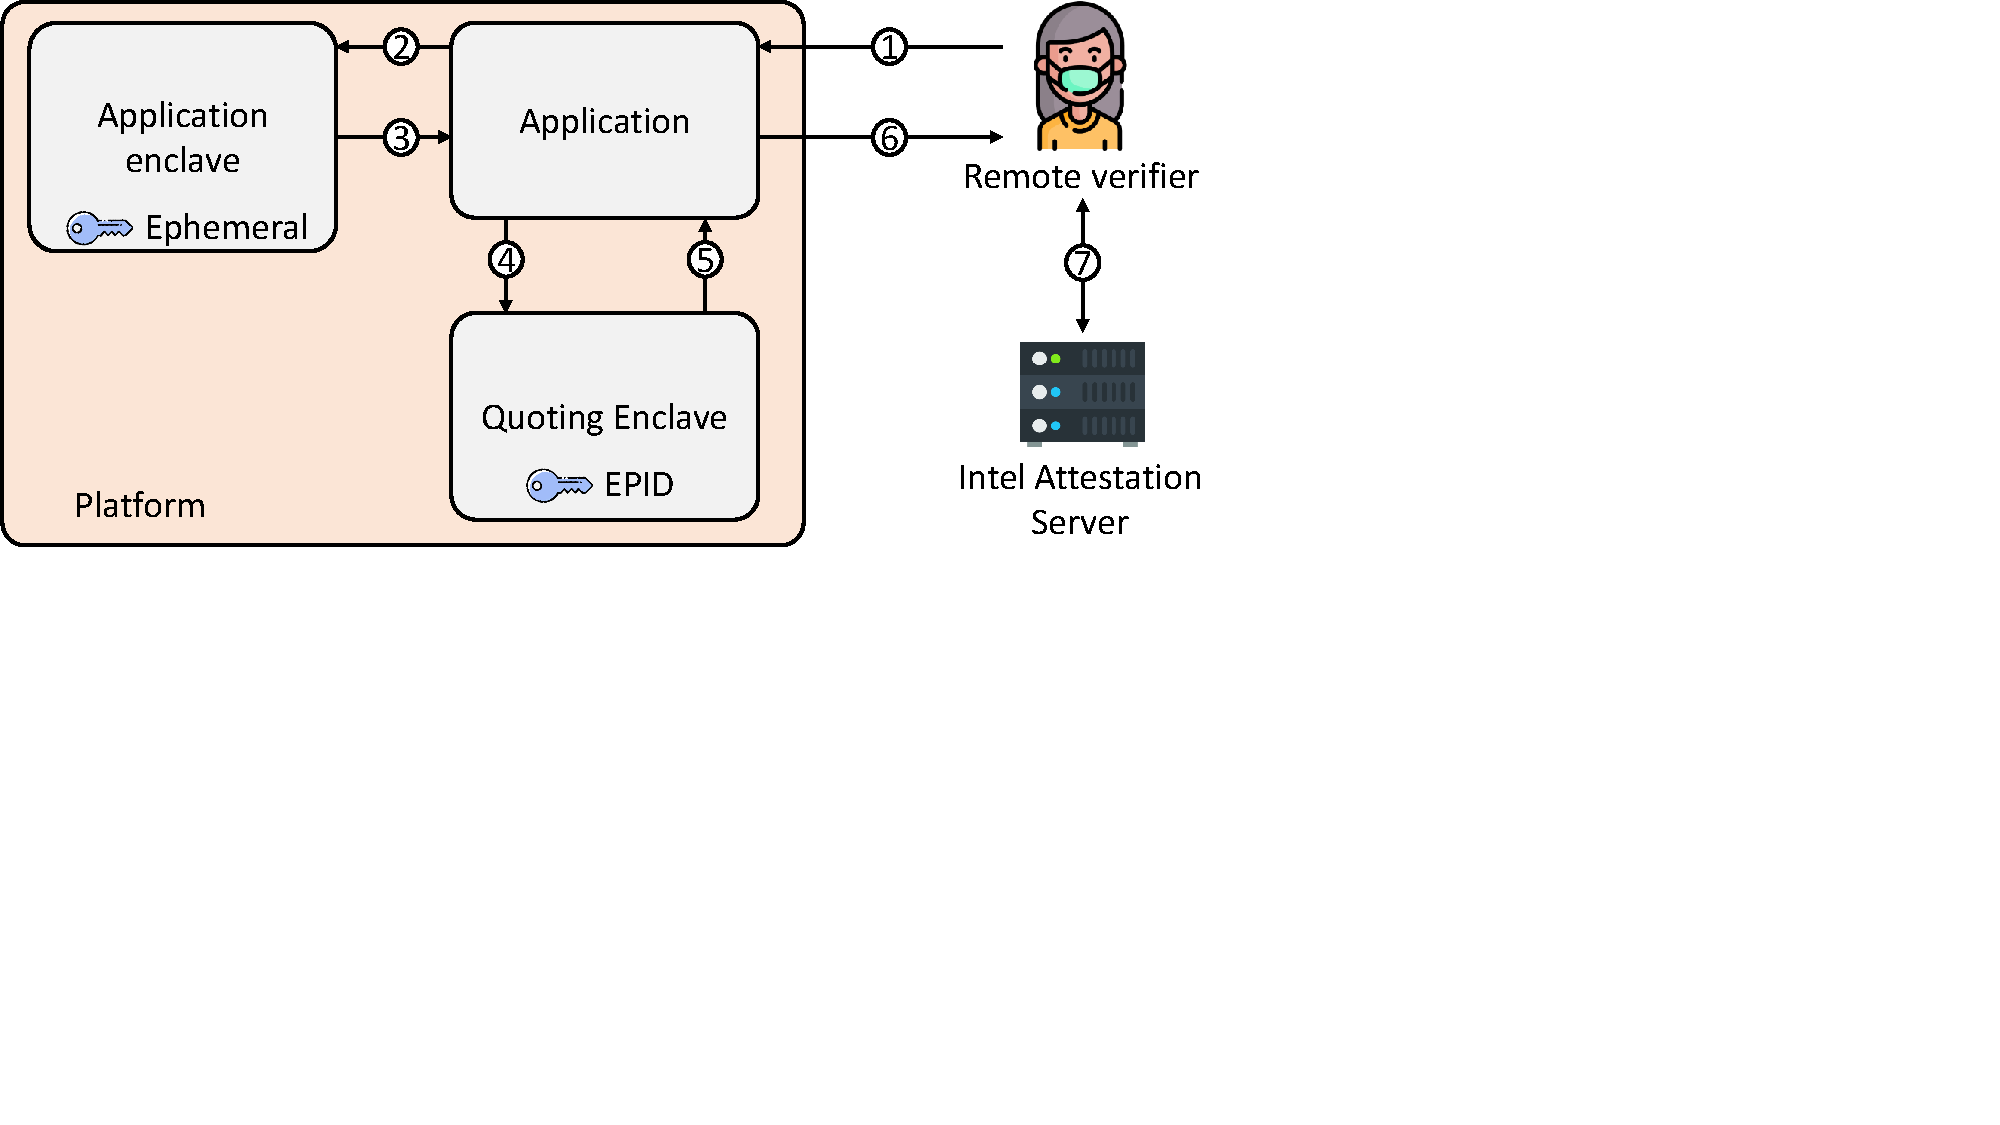
\includegraphics[trim={0 9cm 12cm 0},clip,width=0.9\linewidth]{chapters/background/figures/remote_attestation.pdf}
    \caption[Intel SGX EPID remote attestation example]{\textbf{Intel SGX EPID remote attestation example.} Intel SGX remote attestation example that involves the application enclave, quoting enclave, challenger and Intel attestation server. This figure is a reproduction of the figure in Intel's white paper~\cite{attestation_primitive_all}.}
    \label{fig:ra_bg}
\end{figure}

\subsection{Remote Attestation}
\label{ch:background:SGX:remote}

Remote attestation enables an external verifier to check whether a specific enclave has been correctly instantiated in an SGX protected environment. In the following, we describe the two main classes of remote attestation supported by Intel: i) "enhanced privacy ID" (EPID) attestation~\cite{epid_attestation}, and ii) the recently introduced "data center attestation primitives" (DCAP)~\cite{DCAP}. 

\myparagraph{EPID attestation}

The EPID remote attestation is an interactive protocol between three parties: the remote verifier; the attested SGX platform; and the Intel Attestation Service (IAS), an online service operated by Intel. Each SGX platform includes a system service called \emph{Quoting Enclave} (QE) that has exclusive access to an EPID key. EPID is a group signature scheme that allows a platform to sign objects without uniquely identifying the platform or linking different signatures. Instead, each signer belongs to a "group", and verifiers use the group's public key to verify signatures. EPID supports two modes of signatures. In the fully anonymous mode of EPID, a verifier cannot associate a given signature with a particular member of the group. In Pseudonymous mode, an EPID verifier can determine whether it has verified the platform previously.
One example flow of the EPID remote attestation is shown in Figure~\ref{fig:ra_bg}. The steps are as the following:


\begin{enumerate}
  \item[\one] The remote attestation process starts with the remote verifier who wants to attest to the application enclave running on the remote platform. The remote verifier issues a challenge that is sent to the application. This is because the enclave has no communication capability and depends on the OS or the untrusted application for communication with the outside world. Note that the challenge also includes a nonce for replay protection.
    
  \item[\two] The application is provided with the Quoting Enclave's Enclave Identity. The application relays the remote verifier's challenge to the application enclave.
  
  \item[\three] The enclave generates a manifest that includes a response to the challenge and an ephemerally generated public key to be used by the challenger for communicating secrets back to the enclave. It then generates a hash digest of the manifest and includes it as User Data for the \texttt{EREPORT} instruction that will generate a \texttt{REPORT} that binds the manifest to the enclave. The enclave then sends the \texttt{REPORT} to the application.
  
  \item[\four] The application forwards the \texttt{REPORT} to the Quoting Enclave for signing.
  
  \item[\five]The Quoting Enclave retrieves its Report Key using the \texttt{EGETKEY} instruction and verifies \texttt{REPORT} using the local attestation. It then replaces the MAC over this \texttt{REPORT} with a signature created with a device-specific (private) asymmetric key. The output of this process is called a \texttt{QUOTE}. The Quoting Enclave returns this \texttt{QUOTE} structure to the application. 
  
  \item[\six] The application sends the \texttt{QUOTE} structure and any associated manifest of supporting data to the service challenger.
  
  \item[\seven] The remote verifier sends the \texttt{QUOTE} to the Intel attestation server (IAS) to validate the signature over the \texttt{QUOTE}. IAS then verifies the integrity of the manifest using \texttt{USERDATA} and checks the manifest for the response to the challenge it sent in step \one and send an appropriate response to the remote verifier
 
\end{enumerate} 


The attestation key used by the QE is part of a group signature scheme called EPID that supports two signature modes: random base mode and name base mode, also called "linkable" mode. Both signature modes do not uniquely identify the processor to the IAS, but only a group, like a particular processor manufacturing batch. The difference between them is that the linkable signature mode allows checking whether two attestation requests came from the same CPU. 


\myparagraph{DCAP attestation} Whereas the EPID attestation variant requires connectivity to an Intel-operated attestation service and is limited to pre-defined signature algorithms, the main goal of the DCAP attestation variant is to enable corporations to run their own local attestation services with freely chosen signature types. To achieve this, each SGX platform is, at the time of manufacturing, equipped with a unique \emph{Platform Provisioning ID} (PPID) and \emph{Provisioning Certification Key} (PCK). Intel also provides a trusted \emph{Provisioning Certification Enclave} (PCE) that acts as a local CA and certifies custom Quoting Enclaves that can use freely chosen attestation services and signatures.

DCAP attestation requires a trusted enrollment phase, where the enrolled SGX platform sends its PPID (in encrypted format) to a local corporate key management system that obtains a PCK certificate for the enrolled platform from an Intel-operated DCAP service. After that, the custom Quoting enclave can create a new attestation key that is certified by the PCE enclave on the same platform. The certified attestation key can then be delivered to the corporate key management system that verifies it using the previously obtained PCK certificate. Once such enrollment phase is complete, the custom QE can sign attestation statements that can be verified by a local corporate attestation service without contacting Intel.



\subsection{Side-Channel Leakage}
\label{sec:background:attacks}

Recent research has demonstrated that the SGX architecture is susceptible to side-channel leakage. Secret-dependent data and code access patterns can be observed by monitoring shared physical resources such as CPU caches~\cite{brasser2017software,gotzfried2017cache,moghimi2017cachezoom} or the branch prediction unit~\cite{lee2017inferring}. The OS can also infer the enclave's execution control flow or data accesses by monitoring page fault events~\cite{xu2015controlled}. Many such attacks can be addressed by hardening the enclave's code, e.g., using cryptographic implementations where the data or code access patterns are independent of the key.

The recently discovered system vulnerabilities Spectre~\cite{Kocher2018spectre} and Meltdown~\cite{Lipp2018meltdown} allow application-level code to read memory content of privileged processes across separation boundaries by exploiting subtle side-effects of transient execution. The Foreshadow attack~\cite{foreshadow-usenix18} demonstrates how to extract SGX attestation keys from processors by leveraging the Meltdown vulnerability. 

\subsection{Microcode updates}
As described in Section~\ref{ch:background:SGX:attestation}, during manufacturing, each SGX processor is equipped with two hardware keys. When SGX software is installed on the CPU for the first time, the platform runs a provisioning protocol with Intel. In this protocol, the platform uses one of the hardware keys to demonstrate that it is a genuine Intel CPU running a specific microcode version. It then joins a matching EPID group and obtains an attestation key~\cite{epid_attestation} (or a signing key for the PCE enclave). 

Microcode patches issued by Intel can be installed on processors that are affected by known vulnerabilities such as the Foreshadow attack, as mentioned earlier. When a new microcode version is installed, the processor repeats the provisioning procedure and joins a new group that corresponds to the updated microcode version, and obtains a new attestation key which allows IAS to distinguish attestation signatures that originate from patched processors from attestation signatures made by unpatched processors~\cite{epid_attestation}.